\chapter{Implementation}
\paragraph{}Form Builder implementation in Django using \textbf{Form} class.
\section{Custom Form with predefined fields}
\paragraph{}

Initial Form with four fields :
\begin{itemize}
	\item Name - CharField.
	\item Age - IntegerField.
	\item Address - CharField.
	\item Gender - ChoiceField - Male or Female.
\end{itemize}
\begin{lstlisting}[language=python,numbers=none]
  from django import forms
  class SampleForm(forms.Form):
  	name = forms.CharField()
  	age = forms.IntegerField()
  	address = forms.CharField(required=False)
  	gender = forms.ChoiceField(choices=(('M', 'Male'), ('F','Female')))
\end{lstlisting}
\begin{center}
\fbox{\begin{minipage}{35em}
		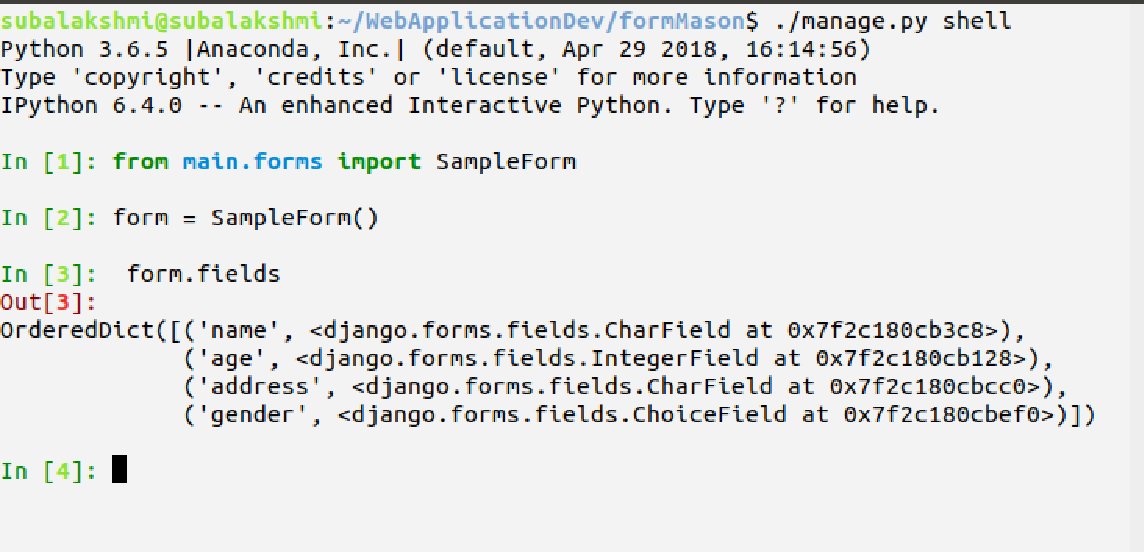
\includegraphics[page=1,scale=0.7]{project/images/orderedDict.pdf}\par
		\captionof{InfoBox}{Ordered dictionary of fields\label{fg:A}}
\end{minipage}}
\end{center}


\section{Adding an extra field to a SampleForm Instance}
\begin{center}
	\fbox{\begin{minipage}{35em}
			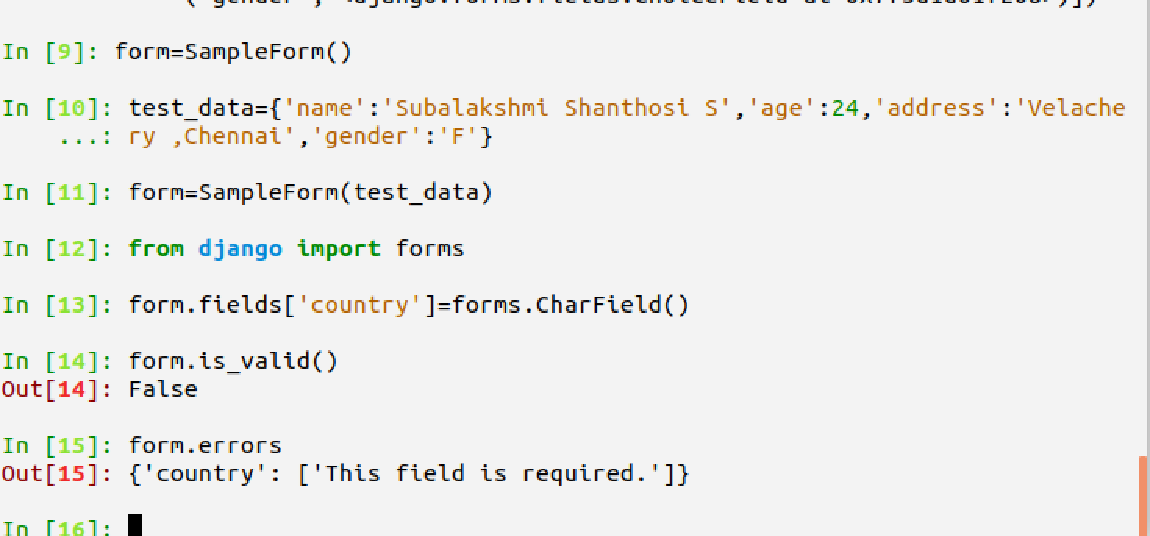
\includegraphics[page=1,scale=0.7]{project/images/includingFieldsForm.pdf}
			\captionof{InfoBox}{Adding new Form field in IShell.\label{fg:B}}
	\end{minipage}}
\end{center}
\newpage
\section{Generating a form out of JSON}

\begin{lstlisting}[language=python,numbers=none]
# main/views.py
class CustomFormView(FormView):
	template_name="custom_form.html"
	#success_url = reverse_lazy('custom_form')

def form_valid(self, form):
	custom_form = FormSchema.objects.get(pk=self.kwargs["form_pk"])
	user_response = form.cleaned_data
	form_response = FormResponse(form=custom_form, response=user_response)
	form_response.save()
	return HttpResponseRedirect(reverse('home'))

def get_form(self):

	# Form structure is predefined with formSchemaIns.schema with the below given json and have done formSchemaIns.save() to load the DB schema
	form_structure = FormSchema.objects.get(pk=1).schema
	#form_structure_json="""{"name":"string","age":"number","city":"string","country":"string","time_lived_in_current_city":"string"}"""
	#form_structure=json.loads(form_structure_json)
	custom_form=forms.Form(**self.get_form_kwargs())
	for key,value in form_structure.items():
	field_class=self.get_field_class_from_type(value)
	if field_class is not None:
		custom_form.fields[key]=field_class()
	else:
		raise TypeError("Invalid field type {}".format(value))

	return custom_form

def get_field_class_from_type(self,value_type):
	if value_type=="string":
		return forms.CharField
	elif value_type == "number":
		return forms.IntegerField
	else:
		return None

def get_context_data(self, **kwargs):
	ctx = super(CustomFormView, self).get_context_data(**kwargs)
	form_schema = FormSchema.objects.get(pk=self.kwargs["form_pk"])
	ctx["form_schema"] = form_schema
	return ctx


\end{lstlisting}
\newpage
\begin{lstlisting}[language=html,numbers=none]
<!--  main/templates/custom_form.html-->
<html>
<head>
<meta http-equiv="content-type" content="text/html; charset=utf-8"/>
<title>Custom Form Demo</title>
</head>
<body>
<h1>Custom Form</h1>
<form action="" method="post">
{{ form.as_p }}
<input type="submit" value="Submit" />
</form>
</body>
</html>
\end{lstlisting}

\begin{lstlisting}[language=python,numbers=none]
 from django.conf.urls import url
 from main.views import CustomFormView
 urlpatterns = [
 url(r'^$', CustomFormView.as_view(), name='custom-form'),
 ]
\end{lstlisting}

\section{A model for our JSON}

Package used : \textbf{django-jsonfield}

$\bullet$ Changes in models:
\begin{itemize}
	\item Form Title as CharField
	\item JSON schema as JSONField of django type.
\end{itemize}
\begin{lstlisting}[language=python,numbers=none]
# A model consisting of two fields namely : Schema in JSON format and form title.
from __future__ import unicode_literals
from django.db import models
from jsonfield import JSONField

class FormSchema(models.Model):
	title = models.CharField(max_length=100)
	schema = JSONField()
\end{lstlisting}

\begin{center}
	\fbox{\begin{minipage}{35em}
			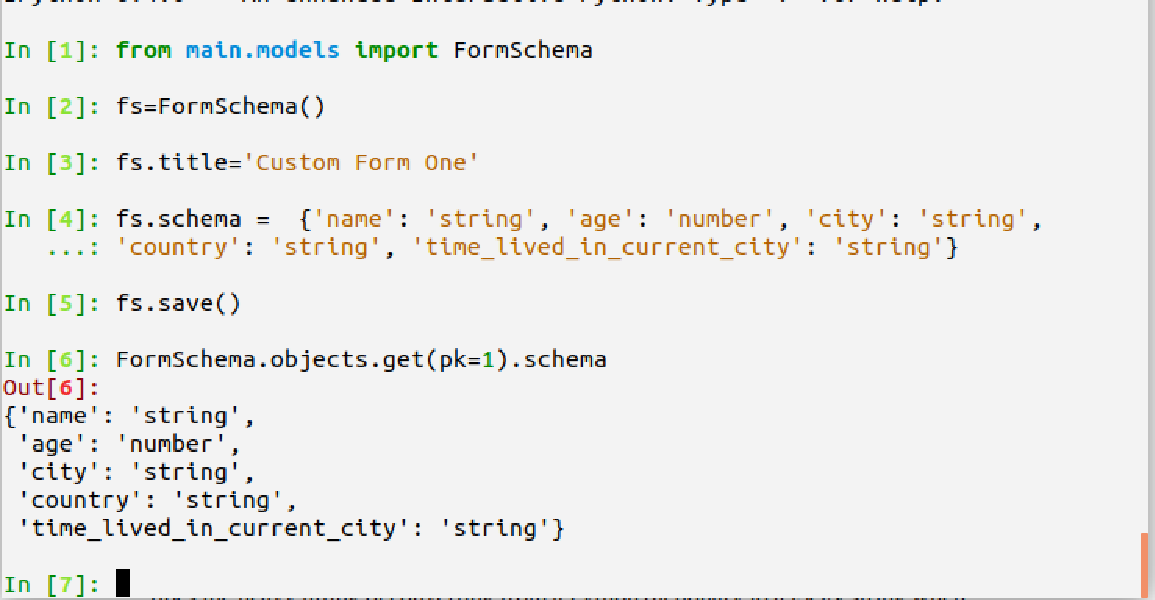
\includegraphics[page=1,scale=0.7]{project/images/formSchemaDefn.pdf}
			\captionof{InfoBox}{Saving changes.\label{fg:C}}
	\end{minipage}}
\end{center}

\section{Creating a better user interface}
\paragraph{}Better user interface by presenting the form\_data in tabular format.\\
Changes in \textbf{settings.py} to include new configuration of templates.\\
\begin{lstlisting}[language=python,numbers=none]
	TEMPLATES = [
	{
	'BACKEND': 'django.template.backends.django.DjangoTemplates',
	'DIRS': [
	os.path.join(BASE_DIR, 'templates'),
	],
	'APP_DIRS': True,
	'OPTIONS': {
	'context_processors': [
		'django.template.context_processors.debug',
		'django.template.context_processors.request',
		'django.contrib.auth.context_processors.auth',
		'django.contrib.messages.context_processors.messages',
		],
	  },
	},
 ]
\end{lstlisting}

\newpage
\paragraph{} Changes in \textbf{base.html}
\begin{lstlisting}[language=python,numbers=none]
	<html>
	<head>
	<meta http-equiv="content-type" content="text/html; charset=utf-8"/>
	<title>Form Mason</title>
	</head>
	<body>
		<a href="">Home</a>
		
		
	</body>
	</html>
\end{lstlisting}
\paragraph{}Changes in \textbf{main/templates/custom\_form.html}

\begin{lstlisting}[language=html,numbers=none]


<h1>Custom Form</h1>
	<form action="" method="post">
	{{ form.as_p }}
	<input type="submit" value="Submit" />
	</form>

\end{lstlisting}
\paragraph{}Changes in \textbf{main/views.py}

\begin{lstlisting}[language=python,numbers=none]
	from django import forms
	from django.views.generic import FormView
	from django.views.generic import ListView
	from main.models import FormSchema
	
	class HomePageView(ListView):
		model = FormSchema
		template_name = "home.html"
	
	class CustomFormView(FormView):
	    template_name = "custom_form.html"
	    
	    def get_form(self):
	    	form_structure = FormSchema.objects.get(pk=self.kwargs["form_
	    pk"]).schema
	    	custom_form =forms.Form(**self.get_form_kwargs())
	    
	    	for key, value in form_structure.items():
	    	field_class = self.get_field_class_from_type(value)
	    
	    	if field_class is not None:
	    		custom_form.fields[key] = field_class()
	   	    else:
	    		raise TypeError("Invalid field type {}".format(value))
	    	return custom_form
	    
	    def get_field_class_from_type(self, value_type):
	    	if value_type == "string":
	    		return forms.CharField
	    	elif value_type == "number":
	    		return forms.IntegerField
	    	else:
	    		return None
\end{lstlisting}
\paragraph{} URL configuration:
\begin{lstlisting}[language=python,numbers=none]
from django.conf.urls import url
from main.views import CustomFormView
from main.views import HomePageView
	urlpatterns = [
	url(r'^$', HomePageView.as_view(), name='home'),
	url(r'^form/(?P<form_pk>\d+)/$', CustomFormView.as_view(),name='custom-form'),
]
\end{lstlisting}
\section{Saving responses of Django Forms}
\paragraph{}Changes to view the responses saved in backend in table:\\
Changes in \textbf{main/views.py}
\begin{lstlisting}[language=python,numbers=none]
class FormResponsesListView(TemplateView):
	def get_context_data(self, **kwargs):
		ctx = super(FormResponsesListView, self).get_context_data(**kwargs)
		form = self.get_form()
		schema = form.schema
		form_fields = schema.keys()
		ctx["headers"] = form_fields
		ctx["form"] = form
		responses = self.get_queryset()
		responses_list = list()
		for response in responses:
			response_values = list()
			response_data = response.response
			for field_name in form_fields:
				if field_name in response_data:
					response_values.append(response_data[field_name])
				else:
					response_values.append('')
			responses_list.append(response_values)
		ctx["object_list"] = responses_list
		return ctx

def get_queryset(self):
	form = self.get_form()
	return FormResponse.objects.filter(form=form)

def get_form(self):
	return FormSchema.objects.get(pk=self.kwargs["form_pk"])
\end{lstlisting}
\paragraph{}Changes in form\_response template to construct table:
\begin{lstlisting}[language=html,numbers=none]


<h1>Responses for {{ form.title }}</h1>
	
		<ul>
		
			<li>{{ response.response }}</li>
		
		</ul>
	

\end{lstlisting}
\paragraph{} Changes in URL configurations:
\begin{lstlisting}[language=python,numbers=none]
from main.views import FormResponsesListView

urlpatterns = [ ... ,

  url(r'^form/(?P<form_pk>\d+)/responses/$', FormResponsesListView.as_view(),name='form-responses'),
]
\end{lstlisting}

\paragraph{}Changes made in home template to include link of newly included view function.

\begin{lstlisting}[language=html,numbers=none]


	<h1>Responses for {{ form.title }}</h1>
	
	<table border="1px">
		<tr>
		
			<th>{{ field_name }}</th>
		
		</tr>
		
		<tr>
		
		<td>{{ field_value }}</td>
		
		</tr>
		
	</table>
	

\end{lstlisting}

\begin{center}
	\fbox{\begin{minipage}{35em}
			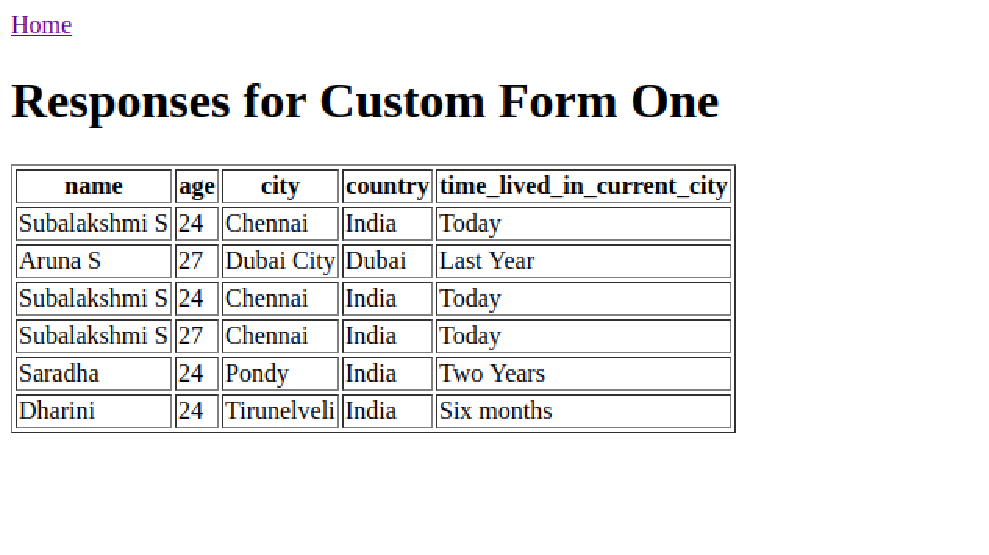
\includegraphics[page=1,scale=0.7]{project/images/improvedView.pdf}
			\captionof{InfoBox}{Tabular view of form responses.\label{fg:D}}
	\end{minipage}}
\end{center}
\section{Designing a form creation interface}
\paragraph{}Changes in \textbf{main/forms.py} to load a JSON which is part of model field got from validation function \textbf{self.cleaned\_data}

\begin{lstlisting}[language=python,numbers=none]
import json
from django import forms
class NewDynamicFormForm(forms.Form):
	form_pk = forms.CharField(widget=forms.HiddenInput(),required=False)
	title = forms.CharField()
	schema = forms.CharField(widget=forms.Textarea())

	def clean_schema(self):
		schema = self.cleaned_data["schema"]
		try:
			schema = json.loads(schema)
		except:
			raise forms.ValidationError("Invalid JSON. Please submit valid JSON for the schema")
		return schema
\end{lstlisting}
\newpage
\paragraph{} CreateEditFormView - class with following methods and instance variables
\begin{itemize}
\item form\_class- NewDynamicFormForm
\item template\_name- create\_edit\_form.html
\item get\_initial - get\_initial Schema if FormSchema object exists else use new schema with title,form\_pk and schema in JSON format , returns initial schema which was formed.
\item  get\_context\_data - same purpose to use inherited reference to CreateEditFormView
\item form\_valid does the following functionality:
\begin{itemize}
	
\item Get form cleaned\_data
\item Check if Any object already found
\item Get Schema old with corresponding pk
\item Set title
\item Set Schema
\item Save form schema
\end{itemize}
\end{itemize}
Flow Alternative
\begin{itemize}
	
\item New Form Flow  - Create new FormSchema
\item Save Schema
\item Return to home.html
\end{itemize}

\paragraph{}Changes in \textbf{create\_edit\_form.html}\\
Include a link to create-edit panel
\begin{lstlisting}[language=python,numbers=none]


<h1>Create/Edit Form</h1>

<form action="" method="post">

<form action="" method="post">

{{ form.as_p }}
<input type="submit" value="Create Form" />
</form>

\end{lstlisting}

\begin{lstlisting}[language=python,numbers=none]
 class CreateEditFormView(FormView):
 	form_class = NewDynamicFormForm
 	template_name = "create_edit_form.html"
 
 	def get_initial(self):
 		if "form_pk" in self.kwargs:
 			form = FormSchema.objects.get(pk=self.kwargs["form_pk"])
 			initial = {
 				"form_pk": form.pk,
 				"title": form.title,
 				"schema": json.dumps(form.schema)
 			}
 		else:
			 initial = {}
 
 		return initial
 
 def get_context_data(self, **kwargs):
 		ctx = super(CreateEditFormView,self).get_context_data(**kwargs)
 		if "form_pk" in self.kwargs:
 			ctx["form_pk"] = self.kwargs["form_pk"]
 		return ctx
 
 def form_valid(self, form):
 		cleaned_data = form.cleaned_data
 		if cleaned_data.get("form_pk"):
 			old_form = FormSchema.objects.get(pk=cleaned_data["form_pk"])
 			old_form.title = cleaned_data["title"]
 			old_form.schema = cleaned_data["schema"]
 			old_form.save()
 		else:
 			new_form = FormSchema(title=cleaned_data["title"],schema=cleaned_data["schema"])
 			new_form.save()
 			return HttpResponseRedirect(reverse("home"))
 
\end{lstlisting}

\begin{lstlisting}[language=python,numbers=none]
  url(r'^$', HomePageView.as_view(), name='home'),
  url(r'^form/(?P<form_pk>\d+)/$', CustomFormView.as_view(),
  name='custom-form'),
  url(r'^form/(?P<form_pk>\d+)/responses/$', FormResponsesListView.
  as_view(), name='form-responses'),
  url(r'form/new/$', CreateEditFormView.as_view(), name='createform'),
  url(r'form/(?P<form_pk>\d+)/edit/$', CreateEditFormView.as_view(),
  name='edit-form'),
  ]
\end{lstlisting}

\newpage

\begin{center}
	\fbox{\begin{minipage}{35em}
			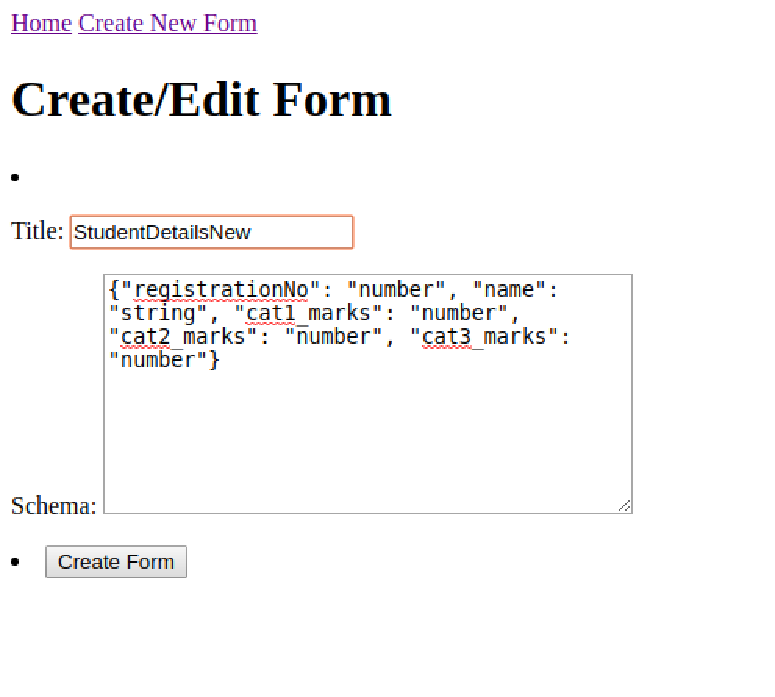
\includegraphics[page=1,scale=0.7]{project/images/jsonSchemaCreation.pdf}
			\captionof{InfoBox}{Form Creation from JSON.\label{fg:E}}
	\end{minipage}}
\end{center}